% Figura Anexo III: cronología de la nueva economía keynesiana (1977-2010): aportaciones arriba, contexto abajo
\documentclass[tikz,border=3pt]{standalone}
\usepackage[T1]{fontenc}
\usepackage[utf8]{inputenc}
\usetikzlibrary{arrows.meta,calc,positioning}
\begin{document}
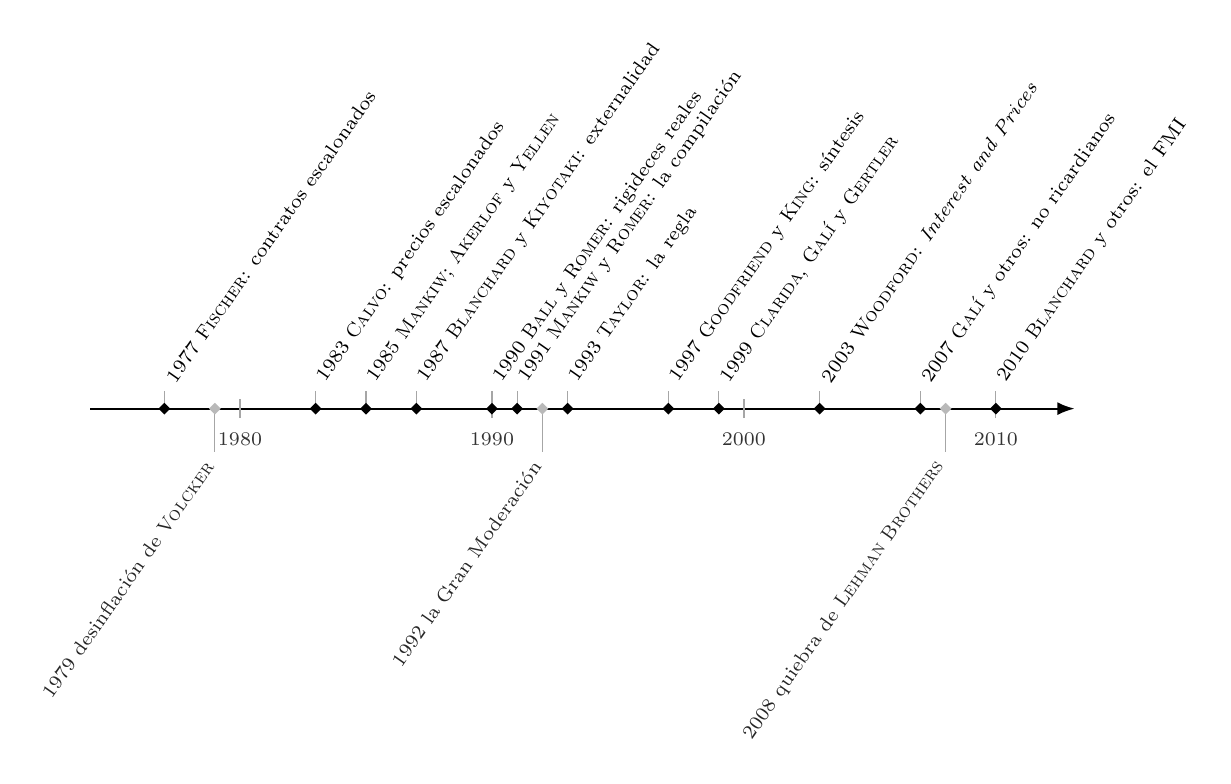
\begin{tikzpicture}[>={Latex[length=2.2mm]}, font=\footnotesize,
  hito/.style={rectangle, fill=black, inner sep=1.5pt, rotate=45},
  ctx/.style={rectangle, fill=gray!55, inner sep=1.5pt, rotate=45},
  arriba/.style={rotate=55, anchor=west, font=\scriptsize},
  abajo/.style={rotate=55, anchor=east, font=\scriptsize, gray!30!black},
  lead/.style={gray!70, thin}]
  \draw[->, thick] (-0.3,0) -- (12.2,0);
  \foreach \y in {1980,1990,2000,2010}{
    \pgfmathsetmacro{\x}{(\y-1975)*0.32}
    \draw[gray!70] (\x,-0.12) -- (\x,0.12);
    \node[font=\scriptsize, gray!40!black, anchor=north] at (\x,-0.18) {\y};
  }
  % Aportaciones (arriba)
  \foreach \y/\txt in {%
    1977/{1977 \textsc{Fischer}: contratos escalonados},
    1983/{1983 \textsc{Calvo}: precios escalonados},
    1985/{1985 \textsc{Mankiw}; \textsc{Akerlof} y \textsc{Yellen}},
    1987/{1987 \textsc{Blanchard} y \textsc{Kiyotaki}: externalidad},
    1990/{1990 \textsc{Ball} y \textsc{Romer}: rigideces reales},
    1991/{1991 \textsc{Mankiw} y \textsc{Romer}: la compilación},
    1993/{1993 \textsc{Taylor}: la regla},
    1997/{1997 \textsc{Goodfriend} y \textsc{King}: síntesis},
    1999/{1999 \textsc{Clarida}, \textsc{Galí} y \textsc{Gertler}},
    2003/{2003 \textsc{Woodford}: \textit{Interest and Prices}},
    2007/{2007 \textsc{Galí} y otros: no ricardianos},
    2010/{2010 \textsc{Blanchard} y otros: el FMI}}{
    \pgfmathsetmacro{\x}{(\y-1975)*0.32}
    \draw[lead] (\x,0) -- (\x,0.22);
    \node[hito] at (\x,0) {};
    \node[arriba] at (\x,0.26) {\txt};
  }
  % Contexto (abajo)
  \foreach \y/\txt in {%
    1979/{1979 desinflación de \textsc{Volcker}},
    1992/{1992 la Gran Moderación},
    2008/{2008 quiebra de \textsc{Lehman Brothers}}}{
    \pgfmathsetmacro{\x}{(\y-1975)*0.32}
    \draw[lead] (\x,0) -- (\x,-0.55);
    \node[ctx] at (\x,0) {};
    \node[abajo] at (\x,-0.59) {\txt};
  }
\end{tikzpicture}
\end{document}
